\documentclass[t]{beamer}

\usetheme{Boadilla}


\usepackage[top=5mm,includehead,headheight=45pt,
             left=1.5cm,bottom=2cm,right=1.5cm,headsep=0.3cm]{geometry} 


\usepackage[T1]{fontenc}
\usepackage{graphicx}
\usepackage{pict2e}
\usepackage{xcolor}
\usepackage{amsmath}
\usepackage[rflt]{floatflt}
\usepackage{graphicx,subfigure,epic,eepic}
\usepackage[most]{tcolorbox}
\usepackage{float}
\usepackage{caption}
\usepackage{fullpage}
\usepackage{hyperref}

%inkscapestuff
\usepackage{import}
\usepackage{pdfpages}
\usepackage{transparent}
\usepackage{xcolor}

\newcommand{\incfig}[2][1]{%
    \def\svgwidth{#1\columnwidth}
    \import{./figures/}{#2.pdf_tex}
}

\pdfsuppresswarningpagegroup=1





\title{Analysis of DUNs (Dynamically unregulated nodes) }
\author{Vaibhav Anand (Intern, CSB)}

\begin{document}


\begin{frame}
\titlepage 
\end{frame}

\begin{frame}
	\frametitle {Three State Formalism}
	The three state formalism with the following rules renders the node with canalising strength 0 incapable of any forward regulation and affecting the state of other nodes at each time step.
	\begin{item}
	\item $ S_j = 1 $ if    $  \sum_{ i } ^ { } adj[i][j] * S_i> 0 $

	\item $ S_j = -1 $ if    $  \sum_{ i } ^ { } adj[i][j] * S_i< 0 $

	\item $ S_j = 0 $ if    $  \sum_{ i } ^ { } adj[i][j] * S_i= 0 $


	\end{item}
	\end{frame}

\begin{frame}

	\frametitle{Story so far}

	Simulating biological networks via three state formalism results in dissapearance of all hybrid states.

\end{frame}



\begin{frame}
	\frametitle{Dynamic InCanalising Strength}

	It quantifies how much activating or inhibhiting regulation and node is under at a certain time step. It is defined as follows for the J'th node
\[   \sum_{ i } ^ { } adj[i][j] * S_i                    \]
Here, $ S_i $ denotes the state of I'th node and adj refers to the adjacency matrix of the network 
\end{frame}

\begin{frame}
	\frametitle{Average DyIncan}
	1000 random inputs are evolved according to the rules of the three state formalism

	and at time steps spaced apart equally, the average of incan values over all the different random input is measured and plotted   
\end{frame}
\begin{frame}
	\frametitle{Evolution of DyInCan}

\begin{figure}[H]\centering

	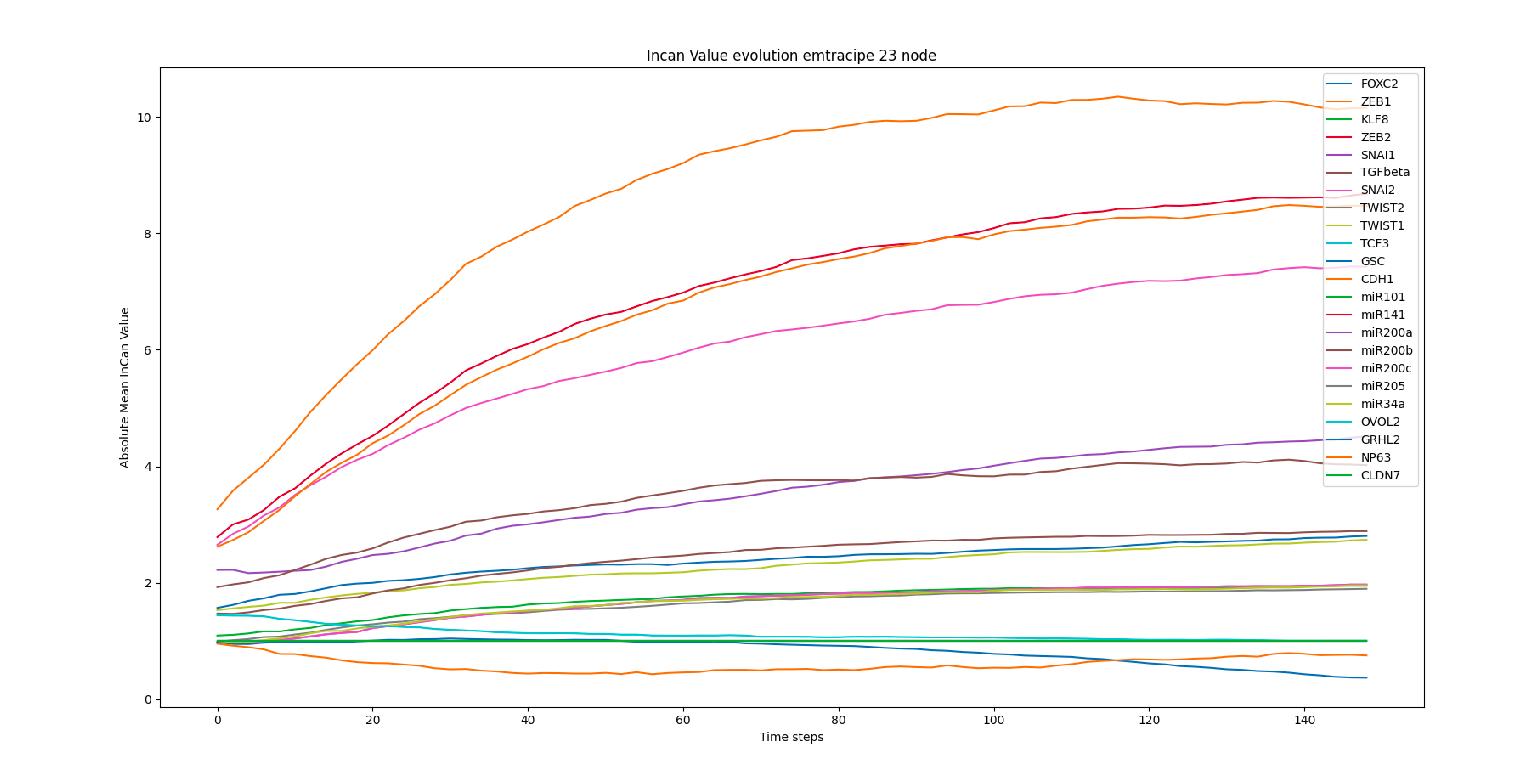
\includegraphics[scale=0.17]{img/emtracipenonnomralised23.png}
	\caption{23 Node EMT network}
\end{figure}
\end{frame}

\begin{frame}
	\frametitle{Ideal Network}
	Ideally, the DyInCan value should eventually become equal to the indegree of the node since all the inhibitory edges (which are between the teams)  should contribute positively to the incan value when one team gets turned off
\end{frame}

\begin{frame}

	\frametitle{Normalized DyInCanValue}

	To compare nodes with different indegrees and to properly measure how "ideal" a node is, I looked at the NormDyInCan Value which is the dynamic incan value divided by the indegree of the node and is defined for a node $ S_j  $ with indegree $ I_j $ as 
	\[   \frac{ |\sum_{ i } ^ { } adj[i][j] * S_i|}{I_j}                    \]
	

\end{frame}


\begin{frame}
	\frametitle{Biological Networks have some nodes which are consistently unregulated}

\begin{figure}[H]
\centering 
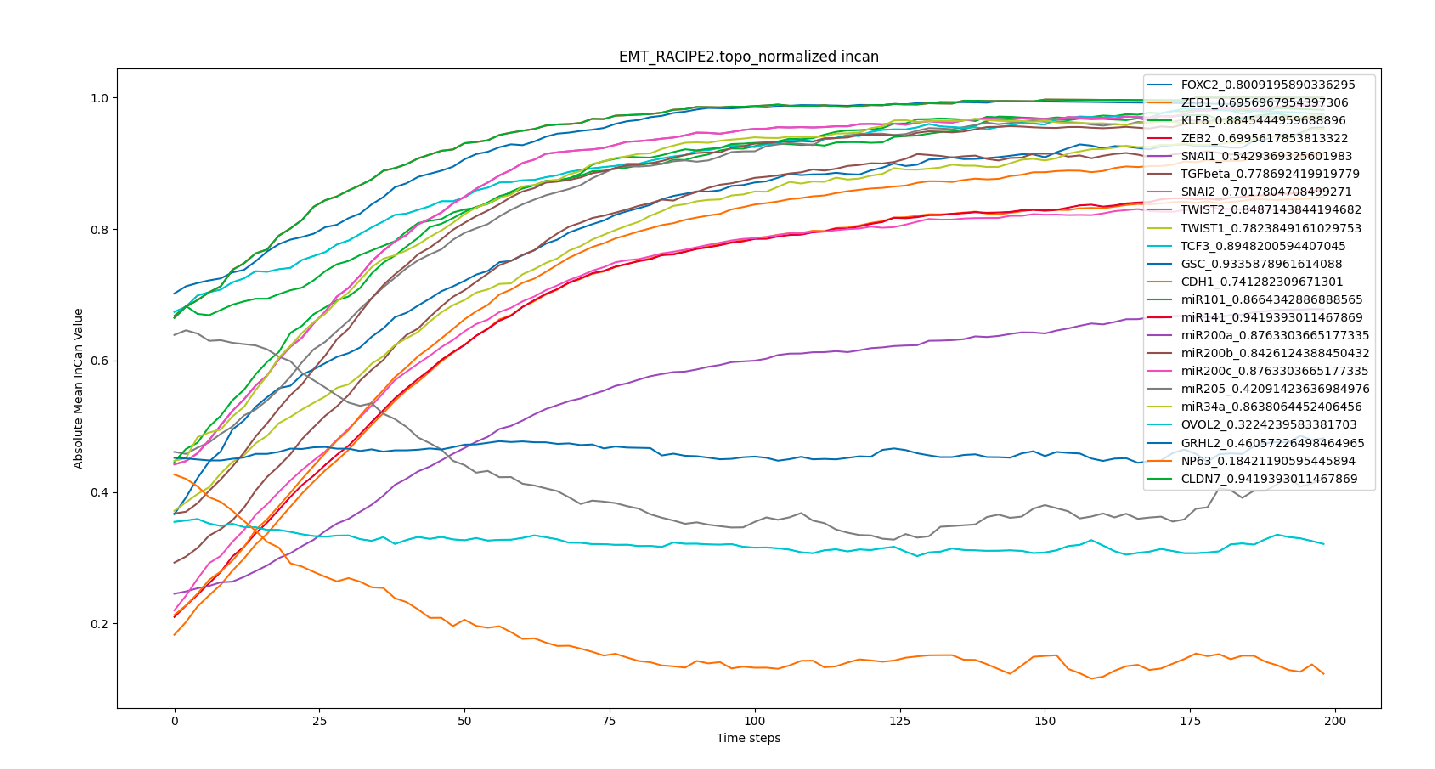
\includegraphics[scale=0.15]{img/emtracipe23incanthreestate.png}

\caption{23 node EMT network, x axis: time, y axis: mean incan}
\end{figure}	
\end{frame}


\begin{frame}
\begin{figure}[H]
\centering

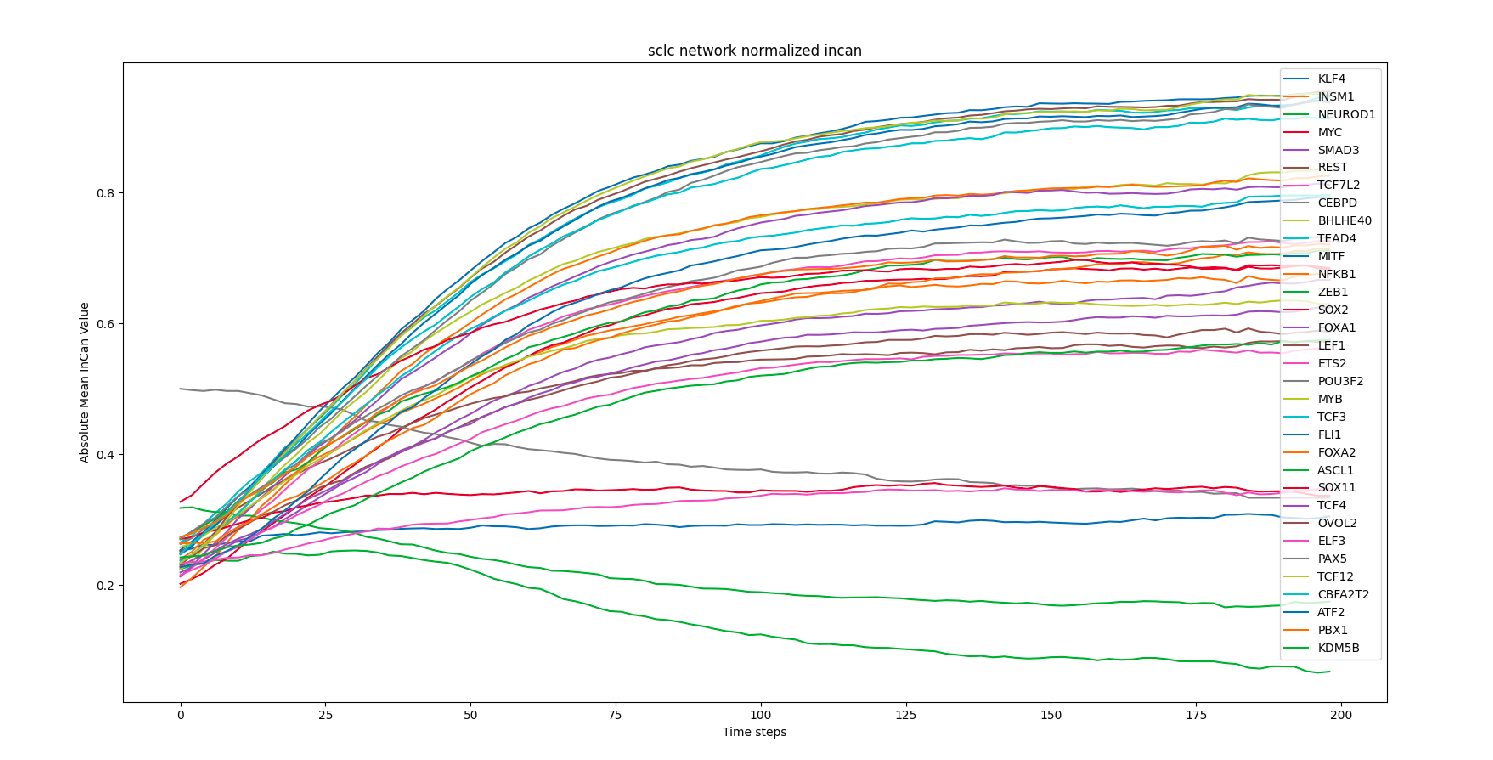
\includegraphics[scale=0.15]{img/sclscnormalizedincan200.png}
\caption{sclc 33 node network, x axis: time, y axis: Mean incan}
\end{figure}
\end{frame}




\begin{frame}
\frametitle{Random networks have more consistently unregulated nodes}

\begin{figure}[H]
	\centering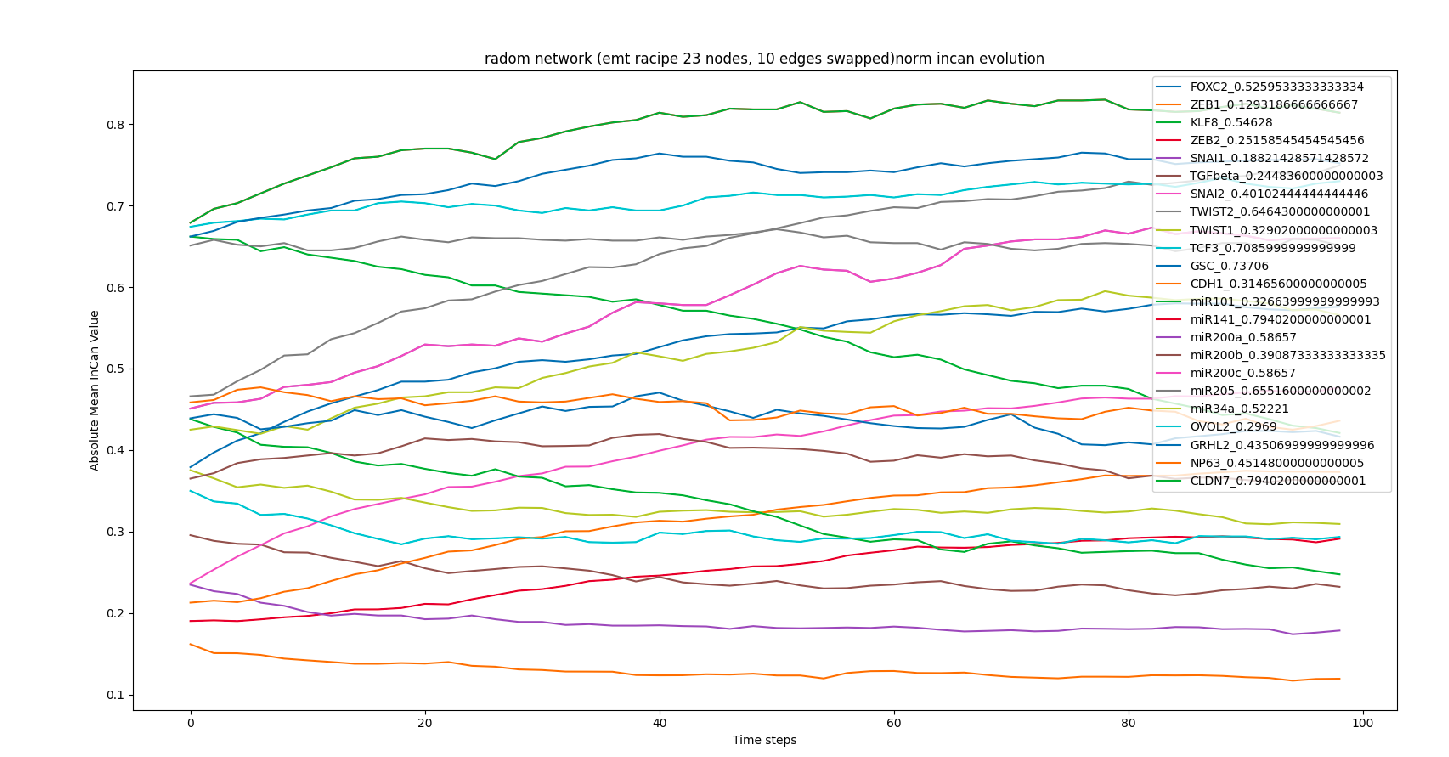
\includegraphics[scale=0.17]{img/randomnetworkemtracipeswap23.png}
	\caption{Random network with 10 edges swapped}
\end{figure}
\end{frame}


\begin{frame}
	\frametitle{Artificial Networks Lack consistently unregulated nodes}

\begin{figure}[H]
\centering 
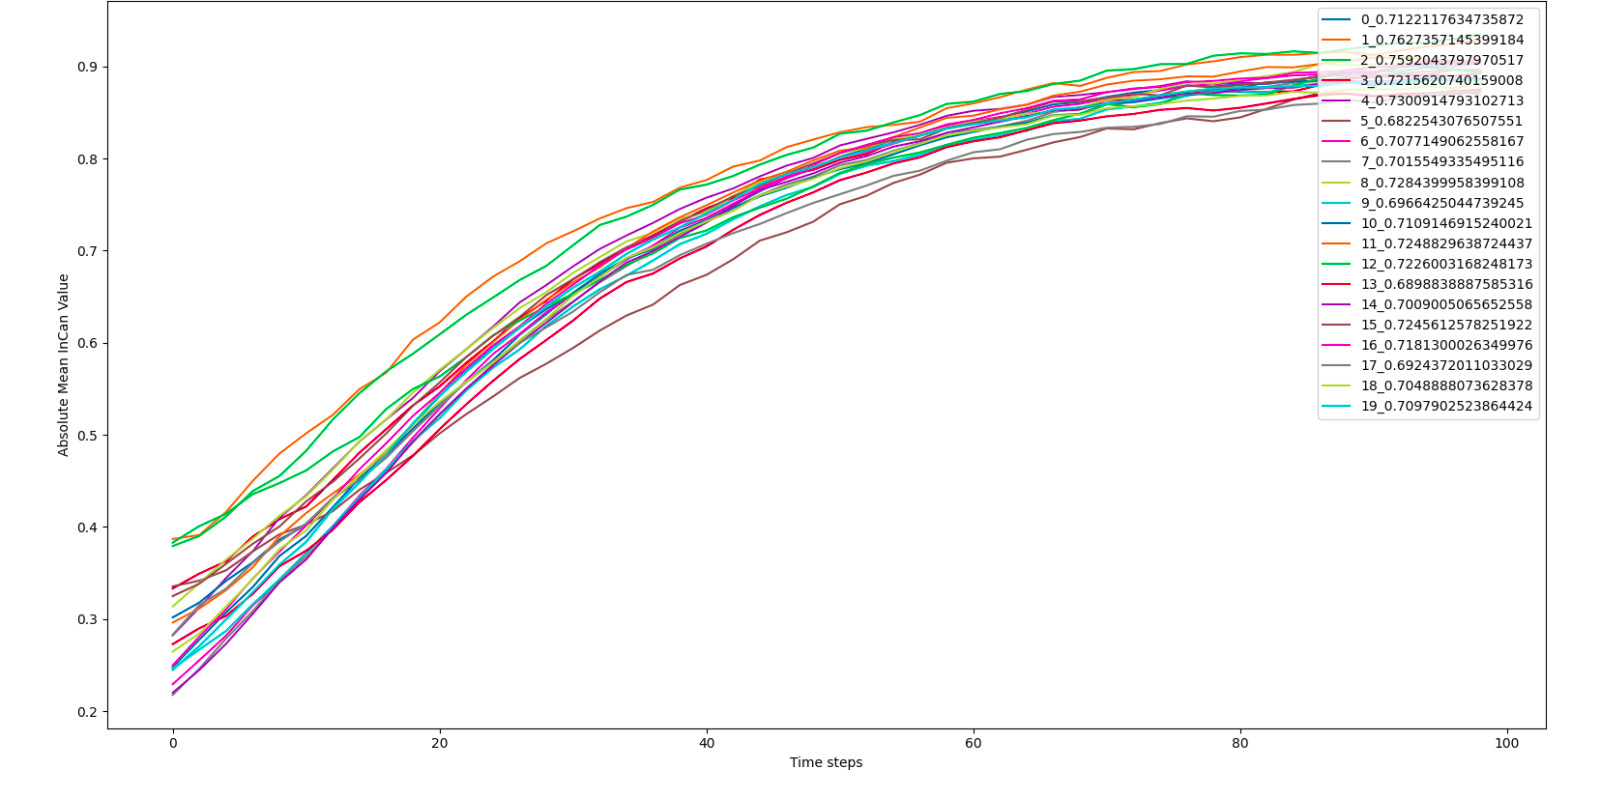
\includegraphics[scale=0.12]{img/artificialnnetworkthreestateincann1.png}
\caption{Artificial network with teams structure }
\end{figure}

\end{frame}


\begin{frame}
	\frametitle{ Static normIncan and Dynamic Incan overlap  }

\begin{figure}[H]
\centering 
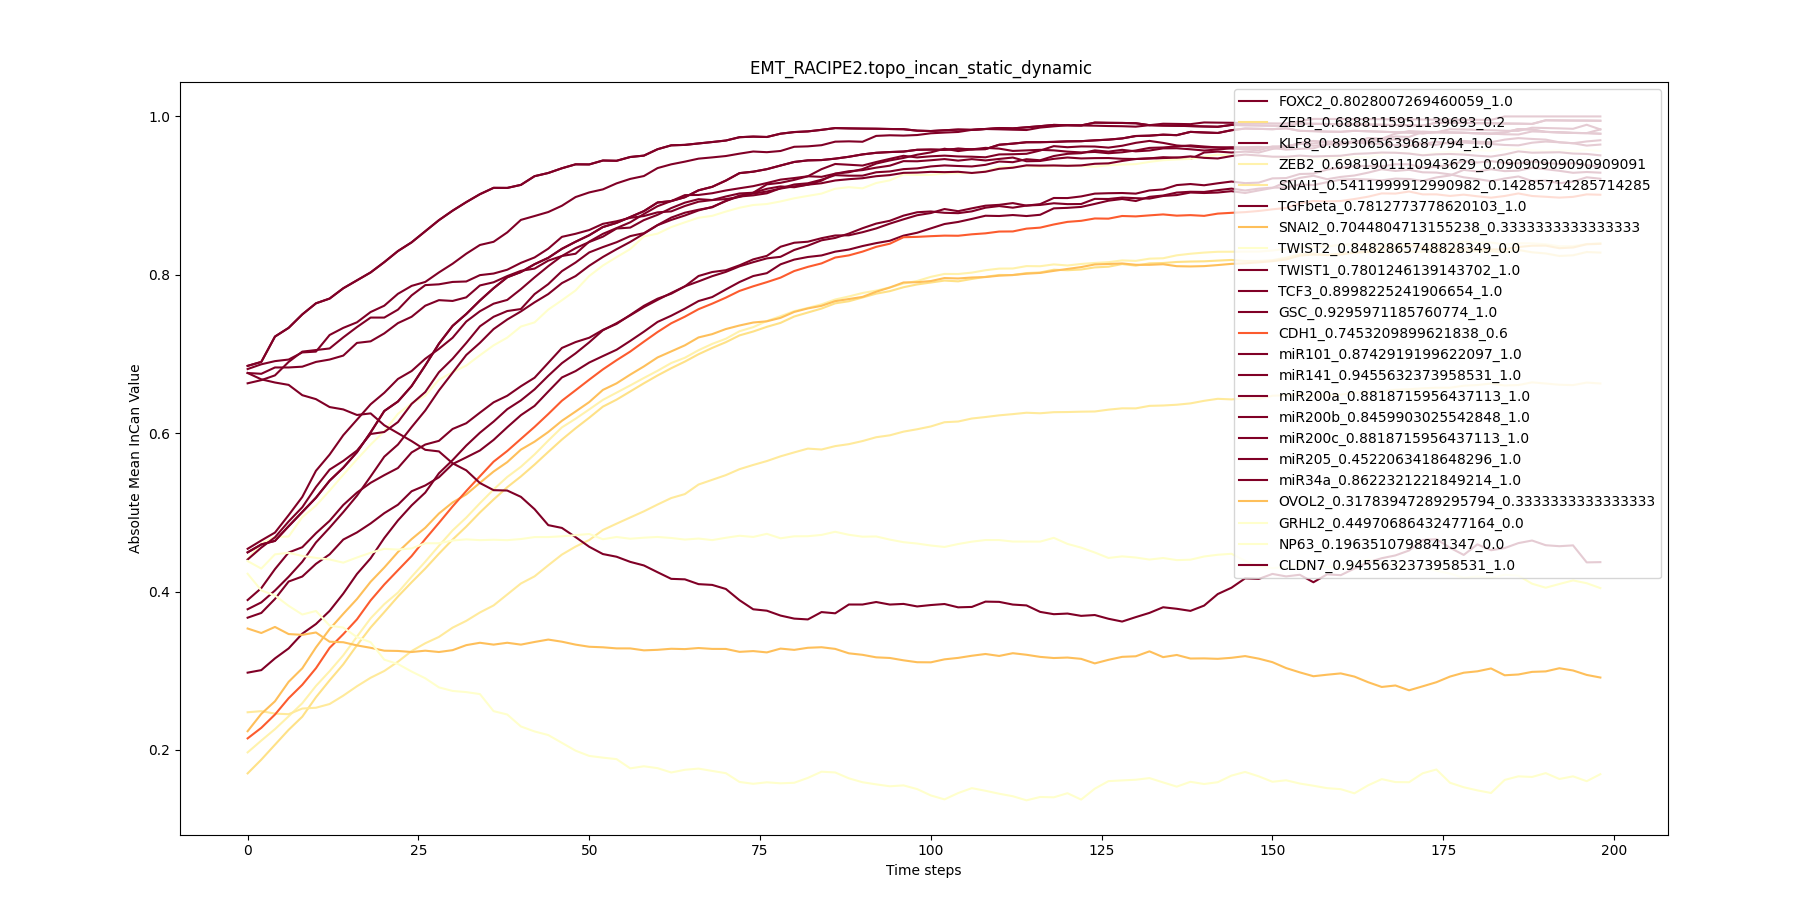
\includegraphics[scale=0.12]{img/static_dyincanemtracipe23.png}
\caption{23 node EMT network}
\end{figure}

\end{frame}


\end{document}

